\documentclass[journal,twoside,web]{ieeecolor}
\usepackage{tmi}
\usepackage{amsmath,amssymb,amsfonts}
\usepackage{algorithmic}
\usepackage{graphicx}
\graphicspath{{images}}
\usepackage{textcomp}
\usepackage[nolist]{acronym}
\usepackage[hidelinks]{hyperref}
\usepackage{float}


\markboth{\journalname, VOL. 01, NO. 01, MARCH 2020}
{TEL22AT1 \MakeLowercase{\textit{et al.}}: Verarbeitung von Gesichtsaufnahmen zur Geschlechterklassifikation als Anwendung neuronaler Netze}

\begin{document}

% Abkürzungen werden hier definiert
\begin{acronym}
    \acro{cnn}[CNN]{Convolutional Neural Network} 
\end{acronym}

\title{Verarbeitung von Gesichtsaufnahmen zur Geschlechterklassifikation als Anwendung neuronaler Netze}
\author{Niklas Herhoffer, Celine Schneider, Andreas Braig
\thanks{Diese Arbeit wurde im Rahmen des Kurses TEL22AT1 erstellt.}
\thanks{Diese Arbeit wurde am 02.03.2025 eingereicht.}  
\thanks{Die Autoren sind Studierende an der Dualen Hochschule Baden-Württemberg Mannheim.}}

\maketitle

% \begin{abstract}
    
% \end{abstract}


\begin{IEEEkeywords}
    Neuronales Netz, Bildsegmentierung, Convolutional Neural Network, Genderklassifikation, Deep Learning
\end{IEEEkeywords}

\section{Einleitung}
\label{sec:introduction}
\IEEEPARstart{D}{iese} Arbeit befasst sich mit der Verarbeitung und Klassifikation von Gesichtsaufnahmen. Die verwendeten Daten bestehen aus Gesichtsaufnahmen von Personen unterschiedlichen Alters. 

Die erste Teilaufgabe der Arbeit besteht in der Segmentierung und Verarbeitung des Datensatzes, um die Gesichtselemente (insbesondere Augen und Mund) in den Bildern einheitlich zu positionieren. Dies wird erreicht, indem ein gleichschenkliges Dreieck mit festen Positionen für die Augen und den Mund im Bild definiert wird. 

Die zweite Teilaufgabe konzentriert sich auf die Klassifikation des Geschlechts der abgebildeten Person. Ein Convolutional Neural Network wird trainiert, um eine binäre Klassifikation zwischen Männlich (0) und Weiblich (1) durchzuführen.

Für die Implementierung wurde die Programmiersprache Python verwendet, unterstützt durch die Bibliotheken OpenCV, numpy und Pytorch.


\section{Stand der Technik}
In diesem Kapitel werden Techniken und Methoden vorgestellt, die für die Verarbeitung von Bildern und die Klassifikation von Gesichtern relevant sind. Dazu gehören Bildsegmentierung, neuronale Netze und Deep Learning-Frameworks, sowie deren Anwendung in der Bildanalyse.

\subsection{Bildsegmentierung}  
Die Bildsegmentierung ist eine Technik der Computer Vision, die ein digitales Bild in einzelne Pixelgruppen unterteilt, um die Objekterkennung und verwandte Aufgaben zu unterstützen.  
Traditionelle Methoden analysieren visuelle Merkmale wie Farbe oder Helligkeit, während moderne Ansätze auf Deep Learning basieren und komplexe neuronale Netze für anspruchsvolle Mustererkennung einsetzen.  
Klassische Verfahren umfassen Schwellenwertmethoden (z. B. Otsu), Kantenerkennung und Clustering-Algorithmen (z. B. K-Means).  
State-of-the-Art-Modelle wie U-Net oder Mask R-\ac{cnn} ermöglichen eine pixelgenaue Segmentierung mit hoher Präzision.  

\subsection{Neuronale Netze und Deep Learning-Frameworks}  
\acp{cnn} spielen eine zentrale Rolle in der modernen Bildverarbeitung.
Sie extrahieren Merkmale durch Faltungsoperationen und ermöglichen effektive Objekterkennung sowie Klassifikation.
Deep Learning-Frameworks wie PyTorch bieten GPU-Unterstützung für beschleunigte Berechnungen, automatische Differenzierung für effizientes Training und flexible Programmierschnittstellen.
Diese Werkzeuge erleichtern die Implementierung komplexer neuronaler Netzarchitekturen für verschiedene Bildverarbeitungsaufgaben.
OpenCV ergänzt diese Fähigkeiten durch effiziente Algorithmen für Filterung, Merkmalsextraktion und Transformationen.

\subsection{Deep Learning in der Bildanalyse}  % Das hier ist irgendwie trash
Deep Learning-Methoden, insbesondere \acp{cnn}, haben die Bildanalyse signifikant verbessert.
\acp{cnn} extrahieren hierarchische Merkmale durch Faltungsoperationen und ermöglichen effiziente Objekterkennung sowie Klassifikation.
Aktuelle Anwendungen umfassen Bildklassifizierung, Objektdetektion und semantische Segmentierung.

Transfer Learning reduziert den Trainingsaufwand durch Nutzung vortrainierter Modelle.
In der industriellen Bildverarbeitung finden Deep Learning-Techniken zunehmend Anwendung, etwa in der automatisierten Qualitätskontrolle und Werkstoffprüfung.
Die kontinuierliche Weiterentwicklung dieser Techniken verspricht weitere Fortschritte, insbesondere in der medizinischen Bildanalyse und industriellen Anwendungen.

\section{Datensatz} \label{sec:dataset}
In diesem Kapitel wird der verwendete Datensatz sowie die damit einhergehenden Herausforderungen beschrieben.

\subsection{Allgemeine Beschreibung des Datensatzes}
Der Datensatz besteht aus ca. 2000 Bildern unterschiedlicher Qualität und Perspektive, die als JPEG-Dateien vorliegen. Zu jedem Bild existiert eine zugehörige Segmentierungsmaske im PNG-Format, welche die relevanten Bildbereiche kennzeichnet. Zusätzlich enthält der Datensatz eine tags.json-Datei, die für jedes Bild das Geschlecht der abgebildeten Person angibt. Die Geschlechterverteilung innerhalb des Datensatzes umfasst ca. 1200 Bilder von Männern und 800 Bilder von Frauen. Dieser Datensatz eignet sich insbesondere für Anwendungen im Bereich der Bildsegmentierung, geschlechtsspezifischen Bildanalysen und Deep-Learning-gestützten Erkennungsaufgaben.

\subsection{Herausforderungen bei der Datenverarbeitung}  
Die Nutzung dieses Datensatzes bringt mehrere Herausforderungen mit sich. Die variierende Bildqualität und unterschiedlichen Perspektiven könnten die Konsistenz der Segmentierung beeinträchtigen und die Generalisierbarkeit von Modellen erschweren. Zudem besteht eine Ungleichverteilung der Geschlechter mit 1200 Bildern von Männern und 800 von Frauen, was zu Verzerrungen in geschlechtsspezifischen Analysen führen kann. Die Qualität und Konsistenz der Segmentierungsmasken ist ein weiterer kritischer Faktor, da ungenaue oder fehlerhafte Masken die Modellleistung negativ beeinflussen könnten. Auch die Labels in der tags.json-Datei könnten Ungenauigkeiten enthalten oder nicht-binäre Identitäten ausschließen, was die Anwendbarkeit in diversen Szenarien einschränkt. Darüber hinaus erfordert die Verarbeitung von 2000 Bildern und Masken erhebliche Rechenleistung und Speicherplatz, insbesondere bei hochauflösenden Daten. 

Falls die Bilder reale Personen zeigen, müssen zudem Datenschutzrichtlinien wie die DSGVO beachtet werden. 

Schließlich könnten je nach Anwendung weitere Herausforderungen auftreten, etwa wenn die Segmentierungsqualität oder Perspektivenvielfalt die Leistung eines Erkennungsmodells beeinträchtigt. Diese Aspekte sollten bei der Vorverarbeitung und Modellentwicklung sorgfältig berücksichtigt werden, um Verzerrungen zu minimieren und robuste Ergebnisse zu erzielen.

\section{Implementierte Lösung}

\begin{figure}[H]
    \centerline{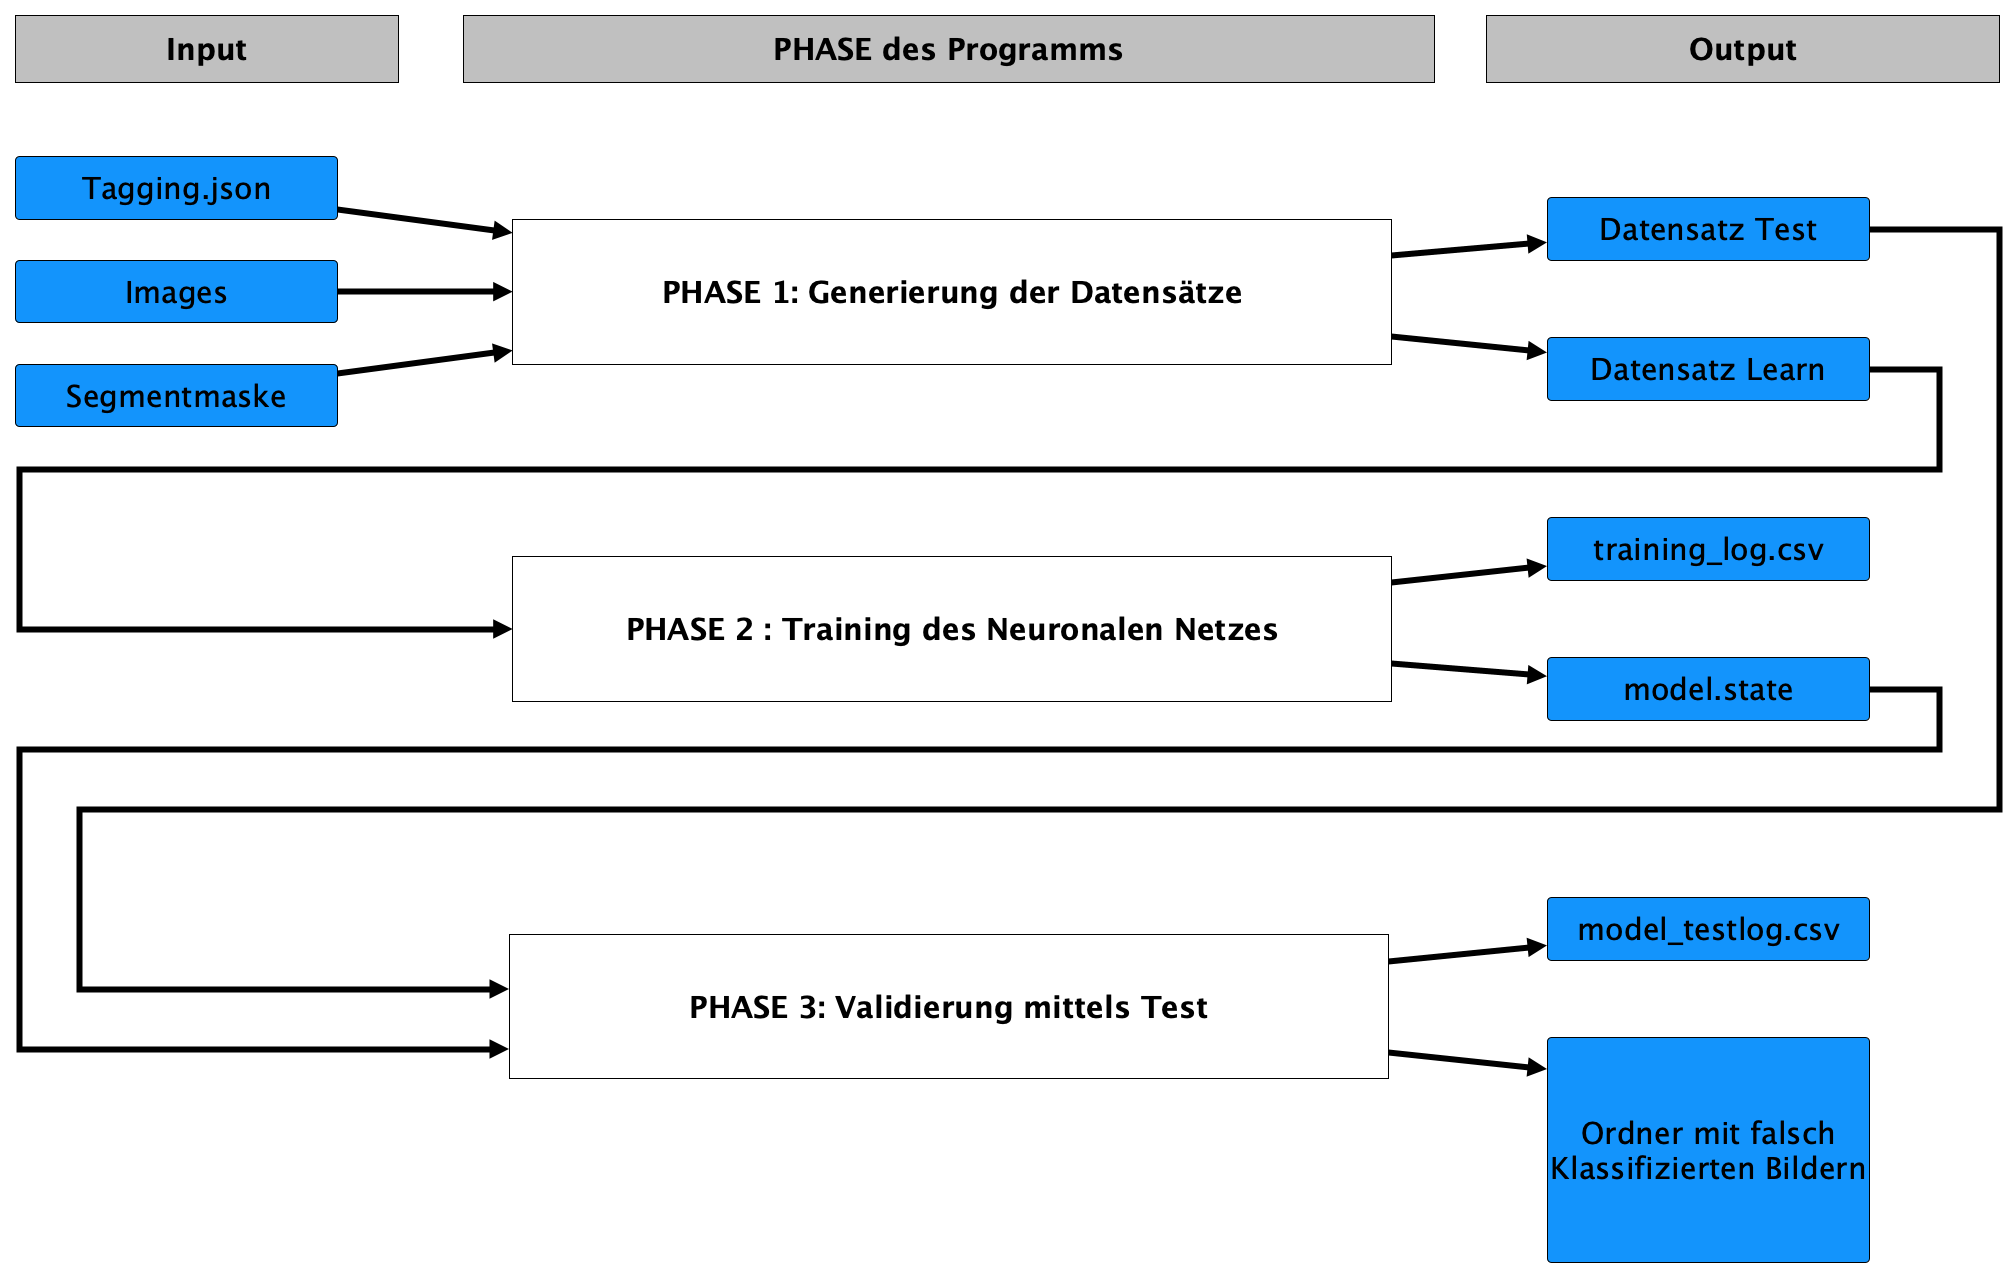
\includegraphics[width=\columnwidth]{Architektur.png}}
    \caption{Darstellung der Programmarchitektur in Form eines Blockschaltbildes}
    \label{fig:architecture}
\end{figure}

Die in Abbildung \ref{fig:architecture} dargetsellte Workflow beschreibt anschaulich die Implementierung des Lösungsvorschlags zu der Aufgabe Geschlechterklassifikation mit dem in Kapitel \ref{sec:dataset} beschriebenen Datensatz.
Im Folgenden wird eine genauere Beschreibung des Lösungsvorgansg gegeben.

\subsection{Get Dataset}
Das Preprocessing übernimmt die zentrale Aufgabe der Vorverarbeitung der Rohdaten für das Training des neuronalen Netzwerks.
Durch die Funktion \texttt{cleanup} wird zunächst sichergestellt, dass sämtliche Datensätze in den Zielordnern gelöscht werden, um eine Vermischung mit einem veralteten Datensatz zu verhindern.
Anschließend werden die Metadaten, einschließlich der Dateinamen und der Geschlechter, aus der \texttt{tag.json} extrahiert und in einem strukturierten 2D-Array gespeichert, sodass die Weiterverarbeitung der Daten erleichtert wird.
Auf Grundlage der so gewonnenen Zuordnungen zwischen Bilddateien und Geschlecht erfolgt die Trennung der Bilddaten in zwei separate Ordner - einen für männliche und einen für weibliche Gesichter.
Im nächsten Schritt wird die Funktion \texttt{freistellen} eingesetzt, um die Gesichter in den Bildern zu extrahieren.
Nach dieser Extraktion erfolgt eine Transformation, die die Gesichter auf eine standardisierte Positionierung von Augen und Mund ausrichtet, um eine konsistente Eingabe für das Modell zu gewährleisten.
Anschließend erfolgt mithilfe der Funktion \texttt{train\_test\_split} die Aufteilung der vorverarbeiteten Bilddaten in Trainings- und Testdatensätze.
Hierbei wird ein zufällig ausgewählter Prozentsatz der Bilder in den Testdatensatz überführt.
Dieser Schritt ist entscheidend, um eine objektive Evaluierung des Modells zu ermöglichen und Überanpassung (Overfitting) zu vermeiden, wie in Abschnitt \ref{sec:overfitting} beschrieben.

\subsection{Preprocessing}

Die Datei \texttt{preprocess.py} dient der Verarbeitung des Datensatzes. Hier werden gezielt Funktionen implementiert, um die gegebenen Ressourcen (Segmentierungsmaske) zu nutzen und die Personen auf den Bildern aufgrund dessen Freizustellen und in die gewünschte Position und Ausrichtung zu transformieren. 

Die Transformation erfolgt über die so genannte affine Transformation. Diese bewirkt, dass geometrische Merkmale nach der Transformation weiterhin erhalten bleiben. Somit bleiben beispielsweise parallele Linien weiterhin parallel.

Zur Berechnung der Transforamtionsmatrix werden die einzelnen Schwerpunkte der Augen und des Musndes benötigt. Diese dienen dem neuronalen Netzwerk später als Ankerpunkte, um für jedes Gesicht immer möglichst die gleiche Ausgangslage zu haben. Zudem wird mit angabe der "Shape" auch die Skalierung der Bilder auf eine einheitliche Größe gebracht.

\subsection{CNN Modell}
Das \ac{cnn} wird verwendet, um das Geschlecht der abgebildeten Person zu klassifizieren. Hierbei kommen mehrere Convolutional Layers und Pooling Layers zum Einsatz, um aus den Eingabebildern tiefere Merkmale zu extrahieren.

% Da eine Anforderung an die Aufgabe darin besteht, die Bilder mit allen vier Kanälen zu verarbeiten muss die Standardfunktion, welche das Bild an das Netz übergibt ersetzt werden.
% Die Standardfunktion konvertiert jedes RGBA Bild in ein Bild ohne Alphakanal, indem dieser abgeschnitten wird. (Schöner Absatz aber hatte unten nix zu suchen.)


\section{Lösungsansätze im Vergleich}
In diesem Kapitel werden fünf Ansätze zur Implementierung des CNN vorgestellt. Insgesamt umfasst die Versuchsreihe 23 trainierte neuronale Netze unterschiedlicher einstellungen und Dimensionen.
Um der Anforderung an diese Dokumentation gerecht zu werden fällt die Wahl auf 5 Modelle die sowohl den Fortschritt, als auch den Wissensgewinn über die Zeit repräsentieren.

\begin{figure}[H]
    \centerline{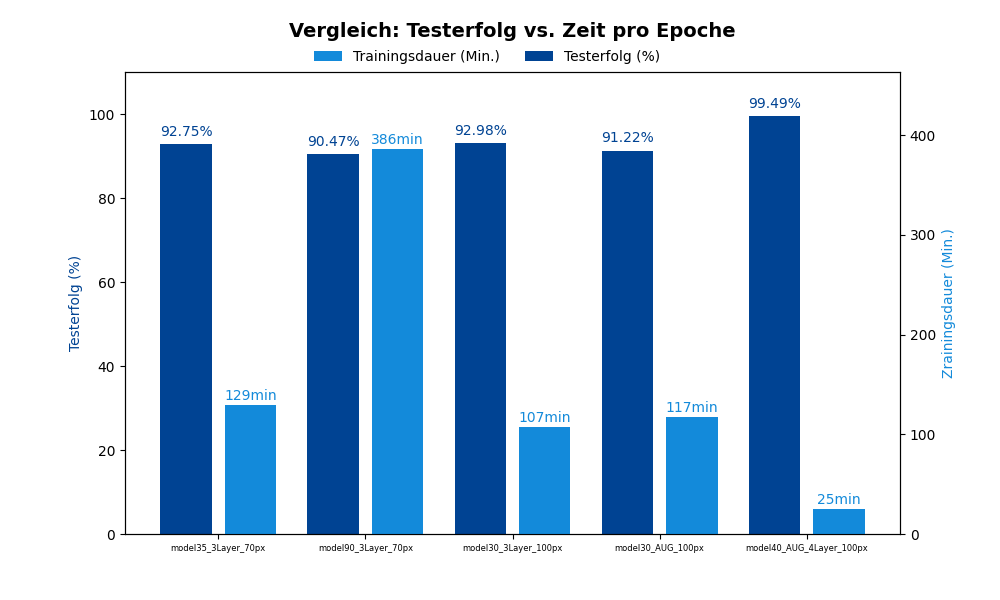
\includegraphics[width=\columnwidth]{Erfolg_Dauer.png}}
    \caption{Vergleichsdiagramm zwischen Erfolgsquote des jeweiligen Modells im Test gegenüber der Dauer einer Trainingsepoche.}
    \label{fig:compareGraph}
\end{figure}

\subsection{Ablauf der Optimierung}
Als Grundlage für das Design des neuralen Netz dient ein im Labor verwendeter Python-Pytorch Code. Dieser Code ist in seinen Parametern ergänzt, um den verwendeten Bildgrößen und Bildkanälen gerecht zu werden. 

Mit dem ersten Prorgammentwurf entsteht das netz "Model35", welches zunächst den besten Wert im Test liefert. Dieses Modell ist mit drei Faltungsebenen und einer Reduktion auf 256*26*35 linearen Datenpunkten ausgestattet.
Es wurde für den Test in 35 Epochen trainiert und liefert $92,7\%$ Genauigkeit im Test (Siehe Abbildung: \ref{fig:compareGraph})

Der erste Ansatz der Optimierung ist die erhöhung der Trainingsepochen. Bei gleichbleibenden Modellparametern wird mit 90 Statt 35 Epochen Trainiert.
Dies hat maßgeblichen Einfluss auf die gesamtdauer, die mit 386min deutlich über den 129min des Vorängers liegt (Siehe Abbildung: \ref{fig:compareGraph}). Dies hat keinen positiven Effekt auf den Erfolg des Tests.

\begin{figure}[H]
    \centerline{\includegraphics[width=\columnwidth]{Erfolg_Größe.png}}
    \caption{Vergleichsdiagramm zwischen Erfolgsquote des jeweiligen Modells im Test gegenüber dem Verbrauchten Speicherplatz.}
    \label{fig:compareSize}
\end{figure}

Der nächste Optimierungsansatz besteht in der erhöhung der Bildauflösung. Die zuvor festgelegten 70px für den Augenabstand werden auf 100px erhöht, was eine Auflösungserhöhung von 210x280 auf 300x400 bedeutet.
Der Augenabstand ist die maßgebliche Größe, um die Segmentierung und Transformation des Bildes durchzuführen.

Diese Erhöhung sorgt für eine Steigerung der Modellkomplexität, da die zuvor verwendeten 256*26*35 Datenpunkte nun auf 256*37*50 erhöht wurden. 
Durch die zusätzlichen Informationen ist eine Stegerung des Erfolges um $0,2\%$ möglich. Durch die Erhöhung der Komplexität und damit auch der Kapazität des Modells auf fast das Doppelte (Siehe Abbildung: \ref{fig:compareSize}), ist eine Betrachtung der Overfitting-Problematik unabdingbar.

Overfittinng beschreibt die Situation, dass das Modell sich an nicht wesentliche Merkmale der Eingangsdaten anpasst. Vereinfacht erklärt: es lernt die Testdaten auswendig und kann dann nicht mehr auf wesentliche Merkmale Klassifizieren.

Um dieser Problematik entgegen zu wirken wurde Data Augmentation in den Programmcode implementiert. 
Diese neue \texttt{apply\_augmenatation} Funktion alterniert die Eingangsbilder der Testdaten in jedem Stapel minimal in Färbung, Helligkeit und Kontrast, um eine Zufallskomponente zu Erzeugen, die das Modell nicht auswendig lernen kann. 

Das Modell (model30\_AUG\_3Layer\_100px) erzielt trotz Augmentation keine Verbesserung des Traingserfolges, sondern verschlechtert diesen mit $91,22\%$. 
Ohne den Augmentation Ansatz zu verwerfen ist die nächste Optimierung die Ergänzung einer weiteren Faltungsebene. 
Dies Reduziert die Linearen Parameter und damit auch die Komplexität des Modells, was sich postiv auf die Traningsdauer auswirkt. 
In einem ersten Test konnte dieses Letzte Modell (model40\_AUG\_3Layer\_100px\_ES) zunächst $94\%$ und in einem zweiten Test $99\%$ erzielen.

\subsection{Diskussion der Lösungsansätze}
Schreib ich noch.
Dieses Modell geht in beiden Grafiken (Abbildung \ref{fig:compareGraph} und Abbildung \ref{fig:compareSize}) eindeutig als Bestes Modell hervor, da es mit geringerer Komplexität und kürzester Trainingsdauer die besten Ergebmisse liefert.


\section{Fazit}
Im Fazit werden die Ergebnisse der Arbeit zusammengefasst und diskutiert. Es wird reflektiert, inwiefern die gesetzten Ziele erreicht wurden und welche Verbesserungspotenziale noch bestehen.








\appendices

% \section*{Appendix und die Nutzung von ergänzenden Dateien}

\section*{Danksagung}

\end{document}
